\documentclass[conference]{IEEEtran}
\IEEEoverridecommandlockouts
% The preceding line is only needed to identify funding in the first footnote. If that is unneeded, please comment it out.
\usepackage{cite}
\usepackage{amsmath,amssymb,amsfonts}
\usepackage{algorithmic}
\usepackage{graphicx}
\usepackage{textcomp}
\usepackage{xcolor}
\usepackage{float}
\usepackage{hyperref}
\def\BibTeX{{\rm B\kern-.05em{\sc i\kern-.025em b}\kern-.08em
    T\kern-.1667em\lower.7ex\hbox{E}\kern-.125emX}}
\usepackage[inline]{enumitem}
\newcommand{\x}{\vspace{2mm}\\}
    
\begin{document}

\title{Using Wake-on-LAN to Manage Home Devices}

\author{\IEEEauthorblockN{Thomas Smith}
\IEEEauthorblockA{\textit{tcs1g20@soton.ac.uk} \\
\textit{University of Southampton}}}

\maketitle

\begin{abstract}
Idle devices result in a large amount of wasted energy within households every day. Through the Wake-on-LAN standard, this paper proposes a convenient way to power your devices on based upon environmental factors. This includes scheduling times, detecting nearby devices, and based upon environmental factors. Users interact with the application using a web API, which allows for easy remote access and control of home devices.
\end{abstract}

\section{Introduction}

It is a common scenario for home devices to be left running all day despite only being in use for a fraction of the time they are awake~\cite{urban_energy_nodate}. The Wake-on-LAN standard offers the ability for many devices to be left in low-power modes and woken using a single central node; by watching for several different events in the local network and environment this project will be able to wake devices exclusively when they are required. By having this central node as a low-power device, this will result in a potentially large reduction in power usage.
\x
Some example use-cases of this application are:

\begin{itemize}[noitemsep]
    \item Scheduling devices to be woken at recurring periods when a device is needed to be used. This allows the user to have a predictable timetable for when the device should be active.
    \item Waking a device when the presence of another device is detected locally. The presence of a local device can infer that the user is nearby and will want to use a different device.
    \item Similarly, waking a device based upon environmental factors can infer the presence of a user but does not require the user to have a mobile device that would need to be detected.
\end{itemize}


\section{Goals}

Table~\ref{tab:goals} shows the goals for this project that are organised using MoSCoW prioritisation to determine what objectives are most important to this project.

\begin{table}[ht]
    \centering
    \begin{tabular}{ | l | p{.65\columnwidth} | l | }
        \hline
         \textbf{No.}
         & \textbf{Goal}
         & \textbf{Priority}
         \\\hline
         1 
         & Wake a Wi-FI device over a local network by sending a magic packet.
         & M
         \\\hline
         2
         & Allow devices to automatically be woken based upon external events.
         & M
         \\\hline
         3
         & Detect devices present in the local WiFi network.
         & M
         \\\hline
         4
         & Detect local Bluetooth devices that are in discoverable mode.
         & M
         \\\hline
         5
         & Allow users to interact with the application using a web HTTP API.
         & M
         \\\hline
         6
         & Use a local database to record any user data.
         & M
         \\\hline
         7
         & Use sensors to track environmental factors. 
         & C
         \\\hline
    \end{tabular}
    \vspace{2mm}
    \caption{The goals of this project using MoSCoW prioritisation.}
    \label{tab:goals}
\end{table}

\section{Research}

\subsection{Wake-on-LAN}

Wake-on-LAN is a network standard that allows remote devices to be turned on by sending a \textit{magic packet} to it. It was first introduced in 1998\footnote{\url{https://web.archive.org/web/20121012155338/http://www-03.ibm.com/press/us/en/pressrelease/2705.wss} (Accessed 09/05/2023)} by the Advanced Manageability Alliance (AMA); this alliance consisted of several large tech companies and was created with the purpose of introducing standards that would helped streamline computer management.
Some examples of standards introduced by the AMA are: Desktop Management Interface\footnote{\url{https://www.dmtf.org/standards/dmi} (Accessed 09/05/2023)}, Alert Standard Format\footnote{\url{https://www.dmtf.org/standards/asf} (Accessed 09/05/2023)}, and Common Information Model\footnote{\url{https://www.dmtf.org/standards/cim} (Accessed 09/05/2023)}.

\vspace{2mm}
\subsubsection{Magic Packet}

A magic packet is a frame with a 102 byte payload that consists of: 

\begin{itemize}[noitemsep]
    \item 6 bytes that are all \textit{0xff}, and
    \item 16 copies of the target device's MAC address.
\end{itemize}

The target device's network interface card (NIC) will be listening for this packet whilst in a low-power mode; when it is broadcast over the network the target device's NIC will send a command to the power supply or motherboard to wake the system up.

\vspace{2mm}
\subsubsection{Limitations}

The Wake-on-LAN standard doesn't include any form of delivery confirmation so there is now way to know if the magic packet sent is received or acted upon. 

\subsection{Waking Non IP-Based Device}

Wake-on-LAN uses an IP packet and as such cannot be sent to devices that don't use IP; these are commonly IoT devices and will use protocols like Zigbee to communicate. Han et al looked at using Zigbee to control power outlets in their paper \textit{Remote-controllable and energy-saving room architecture based on ZigBee communication}~\cite{han_remote-controllable_2009}; devices can be toggled using an IR remote or will automatically be turned off when the power output from the socket falls below a certain threshold.

\subsection{Device Discovery}

\vspace{2mm}
\subsubsection{Over Wireless LAN}

If we are aware of the device's IP address then it is trivial to discover if it is active by sending it a simple request, such as an ARP request, and wait for a response.
\x
Zhou et al describe a system called \textit{ZiFi}~\cite{zhou_zifi_2010}, which uses Zigbee radios to identify the existence of local WiFi networks; this was with the aim of reducing the power requirement needed for a device to discover local WiFi networks. Whilst the use of Zigbee is promising for device discovery, most devices will not come fitted with Zigbee radios. 

\vspace{2mm}
\subsubsection{Bluetooth}

Bluetooth is a short-range, low-bandwidth, low-power wireless communication protocol that is commonly found in battery powered devices. Bluetooth devices organise themselves into \textit{piconets}, which consist of one \textit{master} and up to seven \textit{slave} devices. Each device in the same piconet will have the same frequency hopping sequence that will determined by the master. The formation of a piconet has two steps:

\begin{enumerate}[noitemsep]
    \item \textbf{Inquiry} A master device will discover neighbouring slave devices, and
    \item \textbf{Page} Connections are established between devices.
\end{enumerate}

During the inquiry phase, the master will broadcast an inquiry packet and scan for replies. If a slave wants to be discovered then it will periodically scan for inquiry packets and send a response if they find one. In their paper \textit{A formal analysis of bluetooth discovery}~\cite{duflot_formal_2006}, Duflot et al give a review of the performance of device discovery in Bluetooth v1.2 and v1.1.
A similar analysis of Bluetooth 4.0 is given by Cho et al in their paper \textit{Performance analysis of device discovery of Bluetooth Low Energy (BLE) networks}~\cite{cho_performance_2016}.
\x
Cross et al showed it was possible to discover devices that are not scanning for and replying to inquiry packets in their paper \textit{Detecting non-discoverable Bluetooth devices}~\cite{goetz_detecting_2007}. This was achieved using an `enhanced brute force search attack`; this relied on already knowing the device's MAC address but would still take a considerable amount of time, where most Bluetooth devices would take around 18 hours. 


\section{Design}

\subsection{API}

This application will include a HTTP endpoint that will allow users to access it remotely over the internet.

\subsection{Events}

This section will detail the various events offered by this application that can be used to wake specific devices.

\subsubsection{Schedules}

Users will want to schedule devices to turn on at recurring periods. This application will offer users the ability to set recurring days of the week and times at which a device should be woken.

\subsubsection{Scanning the LAN}

The vast majority of users will have a personal device, such as mobile phone, that will connect to their home router when they're nearby. This means that by listening for when devices join the local network, this application can determine when a user arrives home and can wake the relevant set of devices.
\x
Checking whether a device is in the network can be achieved using an ARP request and assuming that if the device doesn't respond then it can't be in the network.
\x
The user will configure devices to wake when they're personal device joins the network. Some examples would be their PC or various IoT devices around the home.

\subsubsection{Bluetooth}

Bluetooth is a short-range, low-bandwidth, low-power wireless communication protocol that is commonly found in battery powered devices. By allowing this application to search for bluetooth devices, it massvely increases the number of devices we can search for and removes the requirement from the previous section of being in the same LAN.
\x
To initiate a connection, a device will send an \textit{inquiry} message to the target and if the target is in discoverable mode then it will respond. A non-discoverable device will never respond to these messages;
however, the paper \textit{Detecting Non-Discorable Bluetooth Devices}~\cite{} showed that non-discoverable devices can be detected using an `enhanced brute force search attack' as long as you know the device's address. But, this solution is time consuming and wouldn't be a useful addition to this proejct.

\subsubsection{Environment Sensors}

It may be useful for devices to be triggered by environmental factors, such as detecting motion, room temperature, and light.


\section{Implementation}

This section will detail specific implementation details about the application created.

\subsection{API}

The API was written using the FastAPI\footnote{\url{https://fastapi.tiangolo.com/} (Accessed 09/05/2023)} framework due to its simple syntax, built-in support for data validation and serialisation, and its support for OpenAPI documentation that allows developers to easily write documentation and have it hosted to allow users to explore the API.
The use of OAuth2 with JSON Web Tokens meant the API endpoints are secure and only usable by registered users, which allows for the safe, public hosting of this API.

\subsection{Data Storage}

This application will create a local SQLite\footnote{\url{https://sqlite.org/index.html} (Accessed 09/05/2023)} database that will be interacted with using the object relational mapping library SQLAlchemy\footnote{\url{https://www.sqlalchemy.org/} (Accessed 09/05/2023)}. The following tables will be created:

\begin{itemize}[noitemsep]
    \item \textbf{wakeable\_devices} These are the IP-based devices that can be woken over the network by sending a magic packet to them.
    \item \textbf{schedules} These relate a device to many recurring points in time at which the device should be woken up by the application. Each schedule can be toggled individually.
    \item \textbf{watcher\_devices} These are devices that can be searched for locally using the methods described in Section~\ref{subsec:services}. Each device will have a timeout that allows users to restrict how often a detection of this device triggers devices to wake up.
    \item \textbf{watcher\_wakeable\_mapping} This table shows the many-to-many associations between wakeable and watcher devices. Each mapping also stores which mediums should be watched; for example, should the application look for it using Bluetooth.
    \item \textbf{users} This will store the user information to help secure this API. This application will only consider a single admin user.
    \item \textbf{services} Stores information about the background services a user can run and whether they should be run on application startup. The services available are detailed in Section~\ref{subsec:services} and each can be toggled on or off at any point.
    \item \textbf{environment\_listeners} Stores information about each environment listener including what it is watching (noise, light, or temperature), what the threshold value is (to determine when to wake the device), whether this threshold is an upper/lower limit and a reference to the device being woken. 
\end{itemize}

\subsection{Other Details}

\vspace{2mm}
\subsubsection{Docker}

For easy setup, a Dockerfile is provided to allow a user to start the application with a single command without having to manually install any of the dependencies.

\vspace{2mm}
\subsubsection{Environmental Sensing}

The Enviro\footnote{\url{https://shop.pimoroni.com/products/enviro?variant=31155658489939} (Accessed 10/05/2023)} kit and the corresponding Python library\footnote{\url{https://github.com/pimoroni/enviroplus-python} (Accessed 10/05/2023)} was used in conjunction with a Raspberry Pi 4 to detect various environmental factors. 

\subsection{Application Diagram}

Figure~\ref{fig:app-architecture} shows a breakdown of the application architecture. To help improve the maintainability, the applications is broken down into different layers that are abstract from each other, such that any of them could easily be replaced.

\begin{figure}[ht]
    \centering
    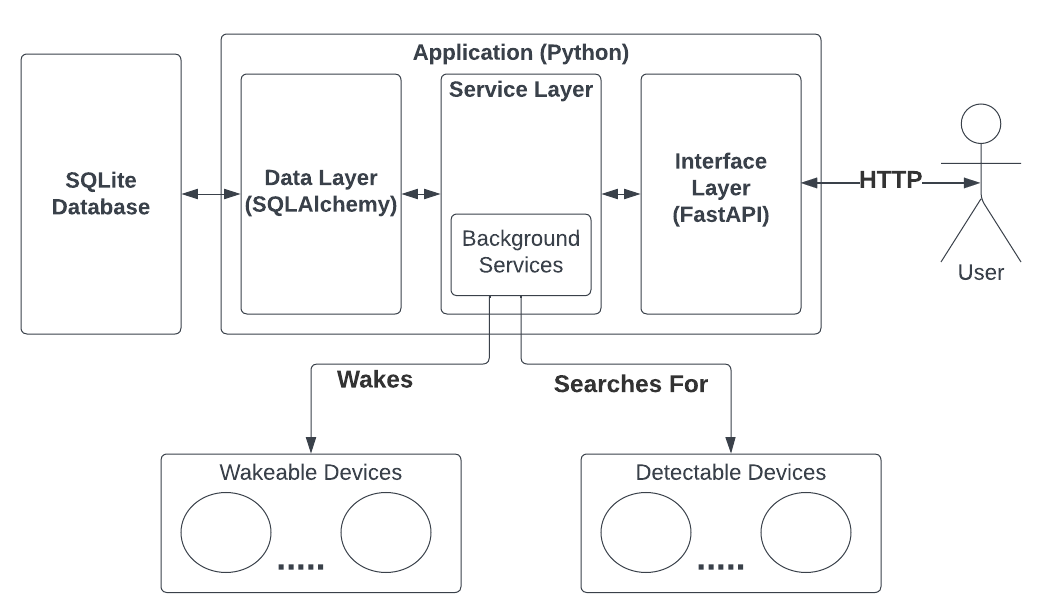
\includegraphics[width=\columnwidth]{assets/application.png}
    \caption{A diagram showing the application architecture.}
    \label{fig:app-architecture}
\end{figure}

\section{Limitations}

Some of the limitations found from this project include:

\begin{itemize}[noitemsep]
    \item devices cannot be remotely turned off through the application and instead rely on the user being able to turn it off themselves,
    \item Wake-on-LAN has no delivery confirmation so my application includes no method for users to verify whether a device was woken; instead it is up to the user to find out themselves, and
    \item The environment sensors used for this application are tightly coupled to a specific piece of hardware for a Raspberry Pi.
\end{itemize}



\section{Conclusion}

In conclusion, this project offers a convenient way for devices to be remotely and automatically woken from low-power modes, which helps contribute to the reduction of unnecessary power usage from idle devices.
\x
An interesting next step would be to consider how this concept could be applied to non-IP devices; this would be specifically prevalent given the recent popularity of IoT devices that are typically \textit{always on}.

\bibliographystyle{ieeetr}
\bibliography{ref}

\end{document}
